\documentclass{styles/llncs} 
%\usepackage{times}
%\usepackage[margin=1in, paperwidth=8.5in, paperheight=11in]{geometry}

\usepackage{geometry}

% bib stuff
\usepackage{cite}
\usepackage{balance}

%\pagestyle{empty}

% math fonts
\usepackage{amstext}
\usepackage{amsfonts} 
\usepackage[cmex10]{amsmath}
% fix the math symbols that the usenix style (mathptmx) changed
\DeclareMathAlphabet{\mathcal}{OMS}{cmsy}{m}{n}
\interdisplaylinepenalty=2500

% paths and extensions for graphic files
\usepackage{graphicx}
\usepackage[outdir=figures/]{epstopdf}
\graphicspath{{figures/}}
% \DeclareGraphicsExtensions{.pdf}

\usepackage{floatflt}
\usepackage[caption=false,font=footnotesize]{subfig}
%\captionsetup[subfloat]{listofformat=parens}

% tables
\usepackage{tabularx}
\usepackage{multirow}
%\usepackage{multicol} 

\usepackage{url}
\usepackage{xspace}
\usepackage[usenames,dvipsnames]{color}

% label the appendices
%\usepackage{appendix}

% reduce space between bib items
% \usepackage{natbib}
% \setlength{\bibsep}{1pt}

% add line numbers for feedback purposes
% \usepackage{lineno}
% \setpagewiselinenumbers
% \modulolinenumbers[1]
% \linenumbers


% should be loaded last (but before algorithm*) -colored links and refs
\usepackage[colorlinks=true, citecolor=OliveGreen, linkcolor=BrickRed, urlcolor=MidnightBlue, final, pdftex]{hyperref}

\hypersetup{
    pdfauthor={Bryan Ford, Miles Richardson, Mainak Ghosh},
    pdfsubject={TorCoin},
    pdftitle={},
    pdfkeywords={Incentive, Monetize, Anonymity, Tor}
}

\usepackage{algorithm}
\usepackage{algorithmic}
\usepackage{subfig}

% space between sections
\renewcommand{\subparagraph}{} % needed to get titlesec to compile
\usepackage[small,compact]{titlesec}
\titlespacing{\section}{0pt}{3mm plus 1mm minus 1mm}{2mm plus 1mm minus 1mm}
% \titlespacing{\subsection}{0pt}{2mm plus 1mm minus 1mm}{1mm plus 1mm minus 1mm}
% \titlespacing{\subsubsection}{0pt}{2mm plus 1mm minus 1mm}{1mm plus 1mm minus 1mm}

% custom commands
\newcommand{\etal}{{\em et al.\ }}
\newcommand{\naive}{na\"{\i}ve }
\newcommand{\point}[1]{\noindent\textbf{#1}.}
\newcommand{\citeme}{\textbf{\color{red}CITE NEEDED! \xspace}}
\newcommand{\checkme}[1][check me]{\textbf{\color{red}NEEDS REVIEW!--{#1} \xspace}}
\newcommand{\todo}[1][check me]{\textbf{\color{red}TODO!--{#1} \xspace}}
\renewcommand{\S}{Section\xspace}
\newcommand{\anote}[1]{{\color{magenta}{#1}}}

% \date{}
\title{TorCoin}
\subtitle{A Proof-of-Bandwidth Altcoin for Compensating Tor Relays}

\author{Bryan Ford \and Miles Richardson \and Mainak Ghosh}

\institute{
	Yale University, New Haven, CT\\
	\email{\{bryan.ford, miles.richardson, mainak.ghosh\}@yale.edu}
}

% Alter some LaTeX defaults for better treatment of figures:
% \renewcommand{\textfraction}{0.07}  % allow minimal text w. figs
% \renewcommand{\floatpagefraction}{0.7}  % require fuller float pages
% \renewcommand{\dblfloatpagefraction}{0.7}   % require fuller float pages

\begin{document}

% \pagenumbering{arabic}

% \clubpenalty=9999
% \widowpenalty=9999 

% space between paragraphs
% \setlength{\parskip}{0.5mm plus 0.25mm minus 0.25mm}

\maketitle
%\thispagestyle{empty}

\begin{abstract}
The scalability of the Tor Anonymity Network currently depends on volunteer relay operators for bandwidth. This is unsustainable. We present a method to compensate Tor relay operators and retain anonymity, without charging clients for access. Our solution relies on two novel concepts. First, we introduce \textit{TorCoin}, an ``altcoin'' that uses the BitCoin protocol to reward relays for contributing bandwidth. Relays ``mine'' TorCoins, then sell them for cash on any existing ``altcoin exchange.'' To verify that a given TorCoin represents actual bandwidth transferred, we introduce \textit{TorPath}, a decentralized protocol for assigning Tor circuits to clients, such that each is privately-addressable but publicly verifiable. [ADD TO THIS WHEN THE PAPER IS DONE]
\end{abstract}

\section{Introduction}

Tor is the most popular deployed anonymous communication system, currently
transferring over 8 GiB/s in aggregate~\cite{tornetmet}. The bandwidth that Tor
requires to function is donated by altruistic volunteers at a cost without any
direct return on their investment. As a result, Tor has primarily grown through
the use social and political means. It is a commonly held belief in the Tor
community that utilizing volunteer resources without providing an incentive to
contribute is not a viable long-term strategy for growing the network. How to
recruit new bandwidth providers to the Tor network while maintaining anonymity
is a well studied problem~\cite{raykova-pet2008, wpes09-xpay, incentives-fc10,
ccs10-braids, acsac11-tortoise, jansen2013lira, johnson2013onions}. However,
none of this work has led to any of a number of practical changes in Tor that
would be required to move to an incentive-based resource model for a variety of
reasons.

This paper has two major goals:
\begin{enumerate}
\item to identify the requirements, challenges, and trade-offs in designing an
incentive scheme for the popular operational Tor Network; and 
\item to propose an incentive-based Tor Network architecture with acceptable
trade-offs while presenting an approach to realizing it with mostly existing
technologies and some additional development.
\end{enumerate}
We hope to illuminate the challenges and research problems in a way that will
provoke useful discussion in the community while creating a useful base for
future research in this area.

We begin in \S\ref{reqs} by identifying the requirements and challenges involved
in designing an incentive scheme for Tor while discussing the potential impacts
that various design decisions may have on the existing network and its
operators. We then propose a technical architecture based on existing
technologies in \S\ref{arch}, discuss related work in \S\ref{rel}, and present
several remaining research problems while concluding in \S\ref{conc}.
\section{Motivation} \label{motivation} Solving the problem of compensating
Tor relays is attractive because it would immediately improve the scalability
of the Tor network. Prior research has not arrived at a satisfactory solution
that operates within the basic requirements of an incentive scheme. We now
outline those requirements.

\subsection{Requirements of an Incentive System} At a basic level, an
incentive system must retain anonymity but have the ability to verifiably
measure bandwidth and reliably distribute payment to the nodes that provide
it. The system must be resilient to adversaries attempting to  identify
clients, or fake bandwidth transfer.

\subsubsection{Anonymity-Preserving Architecture} TorCoin should preserve
anonymity. Currently, no Tor client can recognize another, and no relay can
identify the source or destination of any packet it transfers. Proposed
incentive schemes like Tortoise\cite{acsac11-tortoise} and Gold Star\cite
{incentives-fc10} have compromised clients' anonymity by allowing their
traffic to be identified\cite{jansen2013lira}. An acceptable implementation of TorCoin will at
least retain the anonymity of  the current Tor protocol, but an excellent one
will improve upon it. In a  proportionally differentiated service
\cite{blake1998architecture, dovrolis1999case}  like LIRA
\cite{jansen2013lira} a speed-monitoring adversary can potentially  partition
the anonymity set into clients that are paying for higher speeds,  thus
reducing anonymity.

\subsubsection{Verifiable Bandwidth Accounting} TorCoin needs to measure
bandwidth in such a way that anyone can verify its measurements. Optimally, it
will not require self-reporting or centralized servers, unlike EigenSpeed
\cite{snader2009eigenspeed} or Opportunistic Bandwidth Monitoring
\cite{snader2008tune}. The system should be robust to attackers or groups of
attackers colluding to misreport bandwidth measurements, and the entire
network  should agree on all measurements. TorCoin uses an onion-hashing
scheme to push  ``TorCoin Packets'' to measure the end-to-end throughput of
the circuit rather  than reported network speeds.

\subsubsection{Anonymity Preserving Payment Distribution} Once TorCoin
measures the bandwidth of a given node, it must distribute payment to that
node in a way that preserves anonymity. Specifically, it should not be
possible for anyone to associate a bandwidth payment or measurement with a
specific relay. Combined with the previous constraint, the problem becomes how
to verify bandwidth without identifying its provider.

\subsubsection{Highly-Available, Reliable Transaction Storage} TorCoin must
store sufficient records of previous payments to avoid rewarding a relay twice
for the same bandwidth transfer. We use the BitCoin protocol's distributed
ledger  to track transactions and avoid double spending.

\subsubsection{Scalable and Deployable with Minimal Code Changes} To simplify
deployability, TorCoin should operate mostly as a wrapper around the exiting
Tor clients. It should require minimal changes to the core Tor codebase, and
should not significantly increase latency of requests. A good incentive scheme
should also be scalable to accomodate a large number of users and relays
operating concurrently. Unlike schemes like BRAIDS \cite{ccs10-braids},
TorCoin is designed to be scalable because of its decentralized structure,
small transaction overheads and use of proven protocols  like Bitcoin to
implement some features.

\subsection{Challenges} It is possible to postulate a naive bandwidth-
measurement scheme that uses blinded cryptographic tokens to signify bandwidth
transfer. Suppose in this scheme, a client is able to give each relay a token
for the amount of bandwidth it provides. Relays are then able to convert these
client-signed tokens into some form of an incentive. This scheme is vulnerable
to colluding groups of clients and relays who can simply sign each other's
transfer tokens without actually transferring any bandwidth.

We attempt to counter this through the TorPath scheme that restricts clients'
ability to choose their own path. Assignment Servers bundle large groups of
clients and relays into groups to collectively choose paths. Even if a path
consists entirely of colluding clients and relays (low probability), a built-
in rate-limiting system is able to limit the number of coins such a path can
mint.

% \subsection{TorCoin}

% The problem of incentivizing Tor relays has two main components: bandwidth
% accounting, and payment distribution. 

% \subsubsection{Payment Distribution} TorCoin solves the problem of payment
% distribution without charging clients or relying on a central bank, like
% previous research required. \cite{jansen2013lira} Relays can trade TorCoins for
% cash on any existing altcoin exchange, because TorCoins have inherent value as
% an alternative cryptocurrency. Thus, the network is funded by altcoin investors
% instead of clients, who can continue accessing Tor for free.

% \subsection{TorPath Motivations} TorPath is an anonymous cooperative routing
% scheme that randomly assigns circuits to Tor clients using decentralized,
% cryptographically verifiable methods. It has many potential applications. We
% primarily apply it to the problem of verifying TorCoins, but also briefly
% discuss how it can reduce the latency of the Tor .onion network.

% \subsubsection{Verify TorCoins} TorPath provides a way for circuits to
% anonymously ``sign'' newly minted TorCoins, so that anyone can verify a TorCoin
% actually represents bandwidth transferred. Every circuit has a unique signature,
% generated via contributed randomness, and assigned via consensus. Thus, a
% TorCoin signature does not identify a circuit, but does prove that its existence
% and bandwidth transfer.


% % 
% \subsubsection{Decrease Latency of Tor Hidden Services} TorPath enables a single
% 3-relay ciruit between Tor clients and hidden services (.onion). Currently, a
% Tor Hidden Service (.onion) connection requires two separate 3-relay circuits,
% from both the client and server \cite{torhidden}, so that they cannot identify
% each other. With TorPath, this connection only requires a single 3-relay
% circuit, because the middle relays of the circuit are collectively chosen. So,
% any TorPath middle relay will protect the client from the hidden service, and
% vice versa. This significantly increases throughput of the .onion network, by
% halving the number of relays required for its operation.


% \subsection{Multi-level privacy-preserving protocols in which "clients"
% actually represent multiple levels of stakeholders} % Say an NGO operating in
% Ratistan wants to deploy an anonymizing network ensuring "blanket anonymity" for
% all their local operatives.  They might do this by making all their access
% points transparent Tor proxies (e.g., http://www.adafruit.com/products/1410), so
% that no matter how any of their employees (or even guests on their WLAN) use
% their network, they will be Torified, because that Tor is the only way "out" of
% the NGO's network.  This way if the NGO has good sysadmins, they can help even
% employees or guests who fail to install or use Tor clients properly.  However,
% at least some of the NGO's employees and/or guests might not want to trust the
% NGO's sysadmins completely, and if they just blindly rely on the NGO's
% Tor-proxified access points to do their job and protect their privacy, any
% compromise at the NGO level might compromise any individual. So the individuals
% would also like to run "real" Tor clients on their own machines, and be assured
% that they're protected if either their own Tor client or the NGO's Tor-proxy
% system is uncompromised.  With Tor as it stands, the NGO's Tor proxies would
% interpose a 3-relay Tor path (chosen by the Tor proxy) on every client's
% connection, on top of which each user will interpose an additional 3-relay path
% (chosen by the user's Tor client), for a 6-relay latency to get to anywhere (or
% a 9-relay latency to get to any Tor hidden service, ouch!).  With TorPath, the
% client, NGO, and even a hidden service at the end, could cooperatively choose a
% set of "middle relays" that none of them know or trust but which protect all of
% them from each other simultaneously.

% % In the next section, we outline the TorPath architecture in detail, along with
% some notes on the proposed TorCoin system.

\section{Proposed Architecture} \label{arch}

We now discuss the main components necessary to realize a practical Tor
incentive system while identifying some open research and development problems.

\subsection{Overview}
We propose a system that measures bandwidth contributed to the Tor network to produce incentivise the addition of nodes to the Tor network.

The system measures the bandwidth contributed by each relay in the Tor network and rewards them with a 'TorCoin'. A Torcoin is an AltCoin that uses a bandwidth-intensive protocol as its proof-of-work. Thus, to produce a TorCoin, a relay must have transmitted a certain amount of Tor traffic.

To reduce the system's vulnerability to attackers and possible reduction of anonymity, we also utilize a system of 'Ephemeral Paths' to randomly assign relays to clients.

These TorCoins can then be traded at an exchange for other AltCoins or other goods. This forms the basis of our incentivization scheme. This is different from systems that propose differentiated service\cite{dovrolis1999case, dovrolis2002proportional}, since we do not propose to make the clients pay for access to the network. The coins are a byproduct of the usage of the system.

\subsection{Ephemeral Paths}
The TorCoin system adheres to the following constraints:
\begin{itemize}
  \item No client in the group can generate its own route.
  \item Every resulting route has a unique public key (Route signature).
  \item No client in the group can know the route assigned to another client in the group.
  \item Any interested party can verify that a given public key represents a route assigned to a client in the current group.
\end{itemize}

\subsubsection{Setup}
The Tor directory servers will create the groups using the temporal locality of the clients connecting to them, but also ensure that there is geographical and other diversity in a group. This is to ensure that adversaries cannot deterministically place themselves in a single group by connecting at the same time.

A group consists of the first n = 1000 or so clients that have connected to the Assigning servers. In practice, we expect the number n to be modulated so that groups are being created every 10 seconds or so. Also, we will ensure diversity in the group by ensuring that a group consists of a majority of the Assigning servers. Thus, if there are 10 Assigning Servers in the entire network, a group must consist of atleast 6 of them.


\subsubsection{Route Assignment using Neff shuffles}
Once all the clients have filled up the group, the Assigning Servers in the group initiate the process of route assignment.
\begin{enumerate}
  \item Three groups of two Assigning Servers are chosen from those in the group.
  \item Each group of Assigning servers uses a unique Neff shuffle to create shuffled lists of entry, middle and exit relays. The ith client in the group is thus matched up with the ith entry, middle and exit relay to form a 'route'.
  \item The servers then create a route-signature for each route based on some property of each participant (client and three relays).
  \item Each route-signature is then input into a cryptographic accumulator so that anyone can verify if a route belonged to a group. This accumulator is published in a publicly available log along with the timestamp of the group creation.
\end{enumerate}

Each server then sends each client in the group one piece of data. Eg: The servers that assigned the entry relays send each client its ownentry relay. Similarly, the middle and exit relays and the route signatures are also communicated in the same way. 
For each relay, the servers send an Access Control List. This is a list of all the relays and clients that the relay should accept connections from, as well as the route signatures for each.

In this way, no single server is aware of any client's entire path through the network, preserving their anonymity. Since each relay is confirmed by atleast two servers, it is also robust to rogue servers. 

\subsubsection{Proof of Bandwidth - Onion Hashing}
Once the routes are setup, we can prove bandwidth transfer through the following protocol:
Every m Tor packets, the client sends an extra packet (“the Torcoin packet”) containing an hash attempt likely to generate a TorCoin. Relay A gets it, generates a temporary private key Ka (generated using the route shared key) and hashes the received packet and this key. It then forwards it to B, which does the same thing, with its own private temporary key Kb. Similarly on to C. C can now add its own Kc, and if it generates a hash with a given number of zeros, it can claim to have found a TorCoin.
\begin{verbatim}
Client sends to A: T0 (its hash attempt)
A sends to B     : Hash(T0 + K1) = Ta # K1 is A's temporary private key.
B sends to C     : Hash(Ta + K2) = Tb # K2 is B’s temporary private key.
C computes       : Hash(Tb + K3) = Tc # K3 is C’s temporary private key.
C sends to B     : (Tc, K3) to verify.
B sends to A     : (Tc, K3, Tb, K2) to verify.
A sends to client: (Tc, K3, Tb, K2, Ta, K1) to verify.
Once the client has verified the hash, we can confirm that the data has made a 
round trip through the route. This completes the proof of bandwidth.
\end{verbatim}

\subsubsection{TorCoin}
We can then implement an AltCoin based on the proof-of-work concept in the following manner:
\begin{verbatim}
If (Tc = '000...')
  If the client succesfully verifies the hash
    It adds the coin to the blockchain with the following information:
    0. Timestamp of group.
    1. Client’s public key.
    2. Route Shared key (Lets any other group member verify that the route is 
       genuine. See accumulator.)
    4. TorCoin Hash.
    It then gives 1/3rd of the coin to each of the relays in the route. (If the 
    client is rogue, can we identify and kick the client off?)
\end{verbatim}
This information in the blockchain will enable any interested party to verify if the route came from a legitimate group formed by the directory servers. This can be done by taking the route signature and comparing it with the publicly available accumulators. 

The properties of the Altcoin will then take over, with clients building on the blockchain with more and more TorCoins that they mine through this process.

\subsection{Robustness to attack}
The entire reason for constructing the elaborate ephemeral routes algorithm is to make the Torcoin system robust to attackers.

Due to the random group selection system, it is hard for attackers to deterministically place themselves in a group. To make the system even more secure, the servers can randomize group assignment instead of just taking temporal locality to be the criterion.

In addition, because the attacker needs to control all four components of a route to mint a TorCoin fraudulently, even if the adversaries control up to half the network, there is a probability of only 1/16 that an adversary client gets a path of three colluding relays. In practice, gaining control of half of the entire Tor client and relay network is practically impossible. 

A separate rate-limiting mechanism can be deployed to detect dishonest relays and remove them from the the path selection procedure. An independent verification authority, such as one based on Eigenspeed, could be used to detect these discrepancies.
\subsection{The TorPath Protocol}

\subsubsection{Overview}

The TorPath protocol assigns Tor circuits to clients, overriding Tor directory servers with \textit{assignment servers}, which form decentralized \textit{consensus groups}. The protocol guarantees that no participant on a circuit can identify all other participants, and that each circuit includes a publicly verifiable signature. We use TorPath to ``sign'' each TorCoin, so that anyone can blindly verify a TorCoin by comparing its signature to a global circuit history.

\subsubsection{Requirements}

The TorPath protocol adheres to the following constraints:

\begin{itemize}   
\item No client can generate its own circuit.
\item Every circuit has a unique, publicly-verifiable signature.
\item No client can know the circuit of another client.
\end{itemize}

A consensus group is formed when a majority of the Assignment Servers come
together to assign circuits to clients. Thus, if there are 10 Assignment
Servers in the network, atleast 6 of them must collectively form a group.  The
size of each anonymity group can be modulated to be a number n, i.e., the
group waits until there are n clients to proceed to the next stage. Different
groups can have different values of n to allow each client to choose its own
anonymity level different levels of anonymity. Groups with larger values of n
would provide a larger anonymity set, at the expense of longer circuit setup
times.

\subsubsection{Protocol Description}

The protocol consists of three sequential steps:

\begin{enumerate}
\item \textbf{Group Initialization.} Assignment servers form a \textit{consensus group} by exchanging the public keys of all clients and relays connected to them. 
\item \textbf{Verifiable Shuffle.} The consensus group performs a decentralized, 
verifiable shuffle of all the public keys, resulting in a circuit assignment for
each client.
\item \textbf{Path Lookup.} The assignment servers publish the result of the 
shuffle, such that each client can only identify its entry relay, and each relay
can only identify its neighbors. 
\end{enumerate}


\paragraph{(1/3) Group Initialization}

When a majority of the assignment servers have a sufficient number $n$ of clients
and relays connected to them, they form a consensus group. Clients and relays can specify a minimum $n$ required to join a consensus group. A larger $n$ results in a larger anonymity set, but slower connection speeds while assignment servers
wait for more clients and relays to come online.

A consensus group forms in three separate steps:

\begin{enumerate} 
\item \textbf{Each assignment server} shares its public key with its group members, and
broadcasts the public keys it receives to all clients and relays connected to it. 

\item \textbf{Each client} generates a temporary private and public key pair. It
uses ``onion encryption'' to combine its public key with the public keys of all assignment servers in the group, resulting in a hash that each server can only
partially decrypt. It sends this hash to its own server.

\item \textbf{Each relay} can act as an entry, middle, and/or exit relay, and it chooses which position to assume. In most cases, the number of available relays
will be less than that of clients in a group. To ensure parity between clients
and relays, each assignment server instructs its relays to generate a sufficient
number $n$ keys per position for each client. The relay server uses onion-encryption to generate $n$ hashes from $n$ temporary public keys. It packages them by position and sends them to its assignment server.
\end{enumerate}

The figure below illustrates Steps 2 and 3, after the assignment servers
exchange public keys.

\begin{figure}[htbp]
  \centering
  \subfloat[]{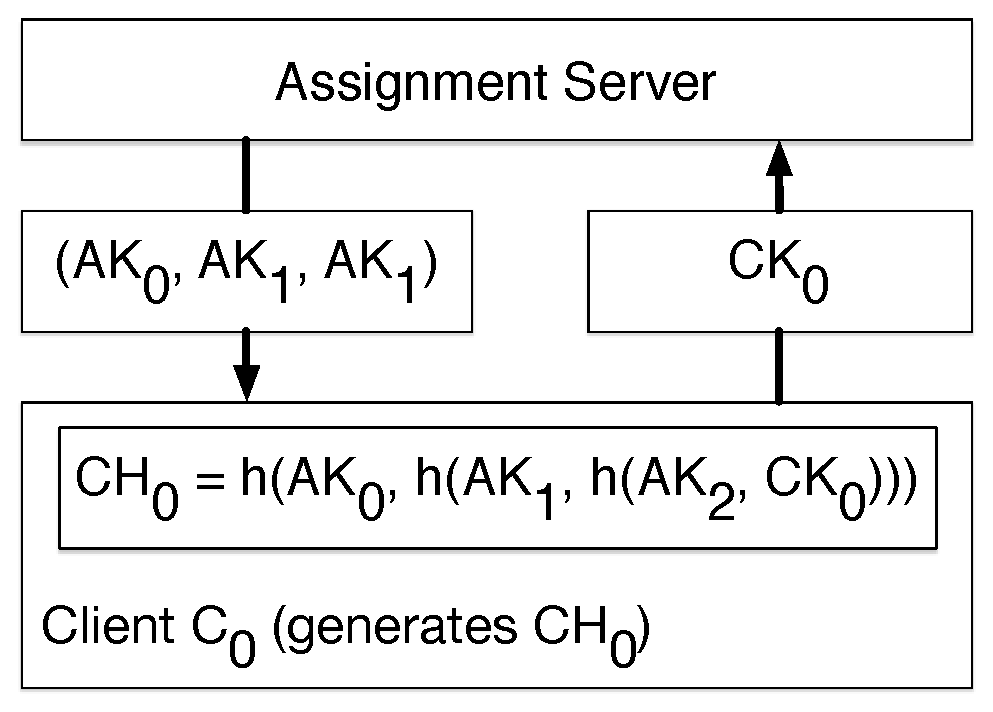
\includegraphics[width=.49\textwidth]{group_formation_2.pdf}}
  \subfloat[]{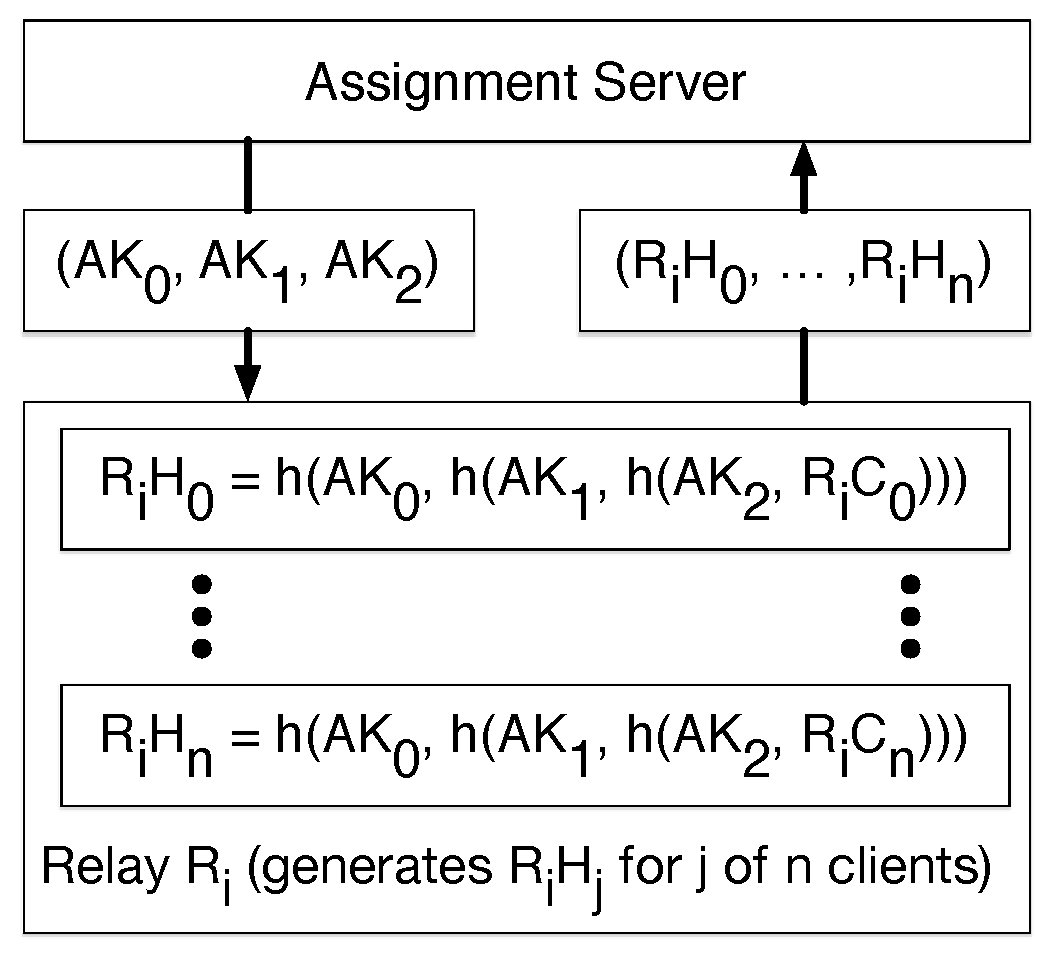
\includegraphics[width=.49\textwidth]{group_formation_3.pdf}}
  \caption{Both relays and clients use onion-encryption to combine their own
  temporary public keys with the public keys of all assignment servers in the group. (a) Client generates one hash. (b) Each relay generates an onion hash for $n$ clients, as instructed by assignment servers, and decides on a position
  for each client.}
\end{figure}

After group initialization, each assignment server constructs a $4 \times n$ matrix for $n$ clients, where each row corresponds to a client and its three relays (see Figure 3a). 

\paragraph{(2/3) Verifiable Shuffle}
Now that the assignment servers have a matrix of circuits for each client, they
``shuffle'' each column so that each client row contains a random triple of
relay public keys. The consensus group collectively shuffles the columns using
a verifiable shuffling algorithm, like the Neff Shuffle \cite{neff2001verifiable}.

\begin{figure}[htb]
\centering
\hspace{\fill}%
\subfloat[htb][Pre-Shuffle]{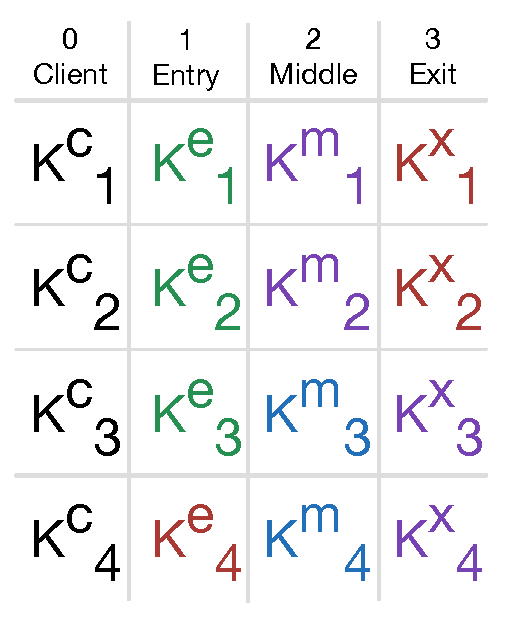
\includegraphics[scale=0.40]{shuffle_1.pdf}}
\hspace{\fill}%
\subfloat[htb][Post-Shuffle]{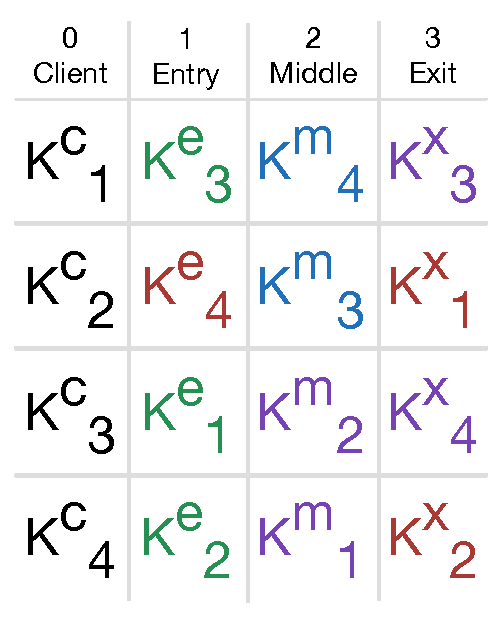
\includegraphics[scale=0.40]{shuffle_2.pdf}}
\hspace*{\fill}%
\caption[bla]{Example matrix shuffle with 4 clients ($K^c_1, K^c_2, K^c_3, K^c_4$) and 4 relays (green, red, purple, and blue). Each row $i$ contains the public keys of a client $K^c_i$ and three relay positions $(K^e_i, K^m_i, K^x_i)$. The
group of assignment servers collectively shuffles the matrix so that each row becomes a circuit.}
\end{figure}

The assignment servers collectively sign and publish the resulting matrix to a public log, accessible by all clients and relays. 

\paragraph{(3/3) Path Lookup}
Path lookup is the final step of the algorithm, where each client obtains the
IP address of its entry relay, and each relay obtains the IP address of its
neighbor(s) on the circuit. The path lookup algorithm ensures that each client
and relay can only receive the IP address of its circuit neighbors.

Each client, and each relay for each client, finds its public key in the matrix.
It uses onion-encryption to hash its IP with the public key of its neighbors,
so that they can find the hash by their public key and decrypt it to find the IP address. 

Consider the $i$th row of the shuffled matrix. Each client and relay finds its 
public key in the $i$th row. It onion-encrypts its IP address with the public
key of its neighbors, and sends it to the assignment server along with its own
public key. Then, the assignment servers perform another shuffle and publish it. At this point, each client and relay can find its neighbors in the matrix by
locating the cells with its public key. Finally, it decrypt those cells using its
private key, revealing the IP address of its circuit neighbor(s).

Now clients have a circuit they can use for Tor.

% {\renewcommand{\arraystretch}{2}
% \begin{tabular}{ c || p{9cm} }
% 		Sender & Message Tuple \\ \hline
% 		Client
% 		&
% 		\begin{flushleft}
% 			$(K_i^c, IP_i^c)$ \\
% 			$IP_i^c$ encrypted with entry relay public key.
% 		\end{flushleft} \\ \hline
		
% 		Entry Relay
% 		&
% 		\begin{flushleft}
% 			$(K_i^e, IP_i^e)$ \\
% 			$IP_i^e$ encrypted with public key of client.	

% 			$K_i^e, 
% 		\end{flushleft} \\ \hline

% 		Middle Relay
% 		&
% 		\begin{flushleft}
% 			....
% 		\end{flushleft} \\ \hline

% 		Exit Relay
% 		&
% 		\begin{flushleft}
% 			....
% 		\end{flushleft} \\ \hline
% \end{tabular}\\


% {\renewcommand{\arraystretch}{2}
% \begin{table}[h]
% \centering
%   \begin{tabular}{ c || p{9cm} }
%   \hline
%   \textbf{Sender} & \textbf{Message Tuple} \\ \hline
%   Client & ($K_{i}^{C}$, {$IP_{i}^{C}$) \\
%   Where $IP_i^c$ is encrypted with the public key of its 
%   entry relay}) \\ \hline
%   Entry relay & ($K_{i}^{E}$, {$IP_{i}^{E}$ encrypted with the public key of 
%   its corresponding client}, {$IP_{i}^{E}$ encrypted with the public key of 
%   its corresponding middle relay}) \\ \hline
%   Middle relay & ($K_{i}^{M}$, {$IP_{i}^{M}$ encrypted with the public key of 
%   corresponding entry relay}, {$IP_{i}^{M}$ encrypted with the public key of 
%   corresponding exit relay}) \\ \hline
%   Exit relay & ($K_{i}^{X}$, {$IP_{i}^{X}$ encrypted with the public key of 
%   corresponding middle relay}) \\ \hline
%   \end{tabular}
%   \caption{Each participant in a circuit sends its message 
%   tuple onion-encrypted to the server. The superscripts refer to the position 
%   of the relay in the circuit and the subscript is the $i^{th}$ row of $M$.}
%   \label{table:message_format}
% \end{table}

% \begin{figure}
% \centering
% 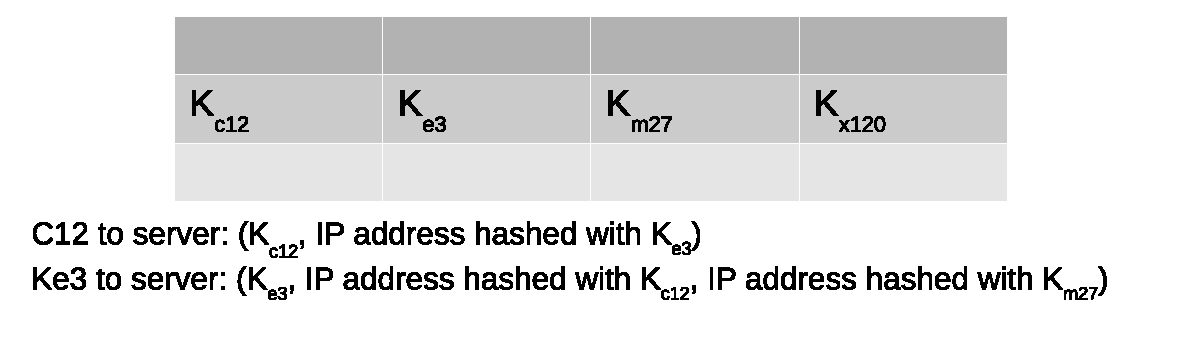
\includegraphics[scale=0.5]{address_lookup.eps}
% \caption{An Example Path Lookup}
% \end{figure}

These tuples are shuffled by the servers again. Each client and relay can then 
decrypt the IP address of their neighbours using their own public key.

The clients then have a circuit which they can use to communicate using the Tor 
protocol.

\paragraph{Circuit Signature} The Circuit Signature of the $i^{th}$ circuit in
a shuffle is the concatenation of the keys in row $i$ of the matrix: $RS_i =
M_{i0}M_{i1}M_{i2}M_{i3}$ This signature will be used in the TorCoin algorithm
to prove that TorCoins are minted only by circuits that have been assigned by
consensus groups.

\subsection{Security Considerations} 

\subsubsection{Anonymity} The TorPath protocol guarantees that no single
server can be aware of the entire circuit of any client. The anonymity set
comprises of all the clients that participate in a particular consensus group.
Groups have various sizes, allowing clients to choose the anonymity threshold
they require.

\subsubsection{Random Group Selection} The TorPath protocol increases
robustness of TorCoin to attackers. Its random group selection system prevents
attackers from deterministically placing themselves in a group. We assume that
atleast one of the assignment servers in the group is honest. In this case,
the group as a whole is able to retain privacy and anonymity. We could make
the system even more secure by randomizing group assignment, instead of just
taking temporal locality to be the only criterion.



% % Next we will descibe the consensus groups and Neff shuffle in more detail.

% % \begin{figure}[H] %   \centering %
% 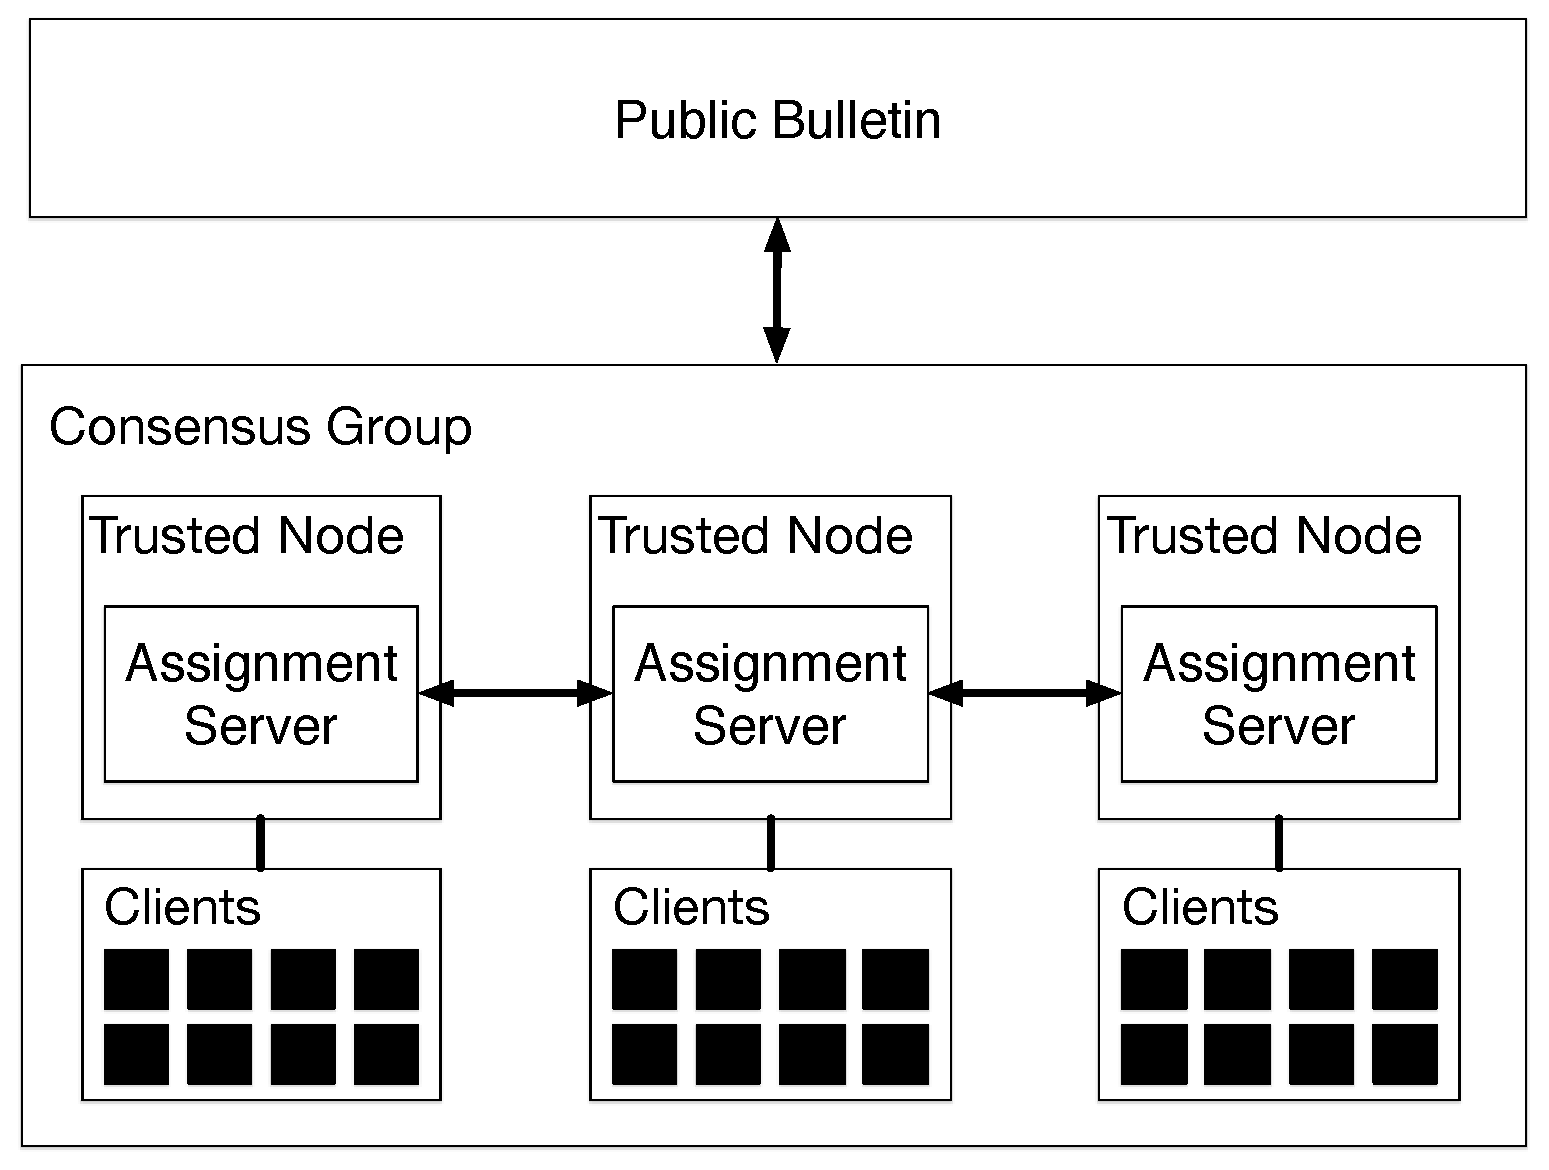
\includegraphics[scale=0.3]{torpath_grouping.pdf} %   \caption{TorPath Consensus
% Group Formation.} % \end{figure}

% % \subsubsection{Group Formation} % An assignment server joins a group when it
% reaches a sufficient number of clients. In practice, we expect the number to be
% modulated so that groups are being created every 10 seconds or so. To ensure
% diversity, groups must include a majority of the assignment servers on the
% network. For example, if there are ten of assignment servers on the entire
% network, a consensus group requires at least six.

% % Once a consensus group exists, it splits into three decentralized shuffle
% % sets, each responsible for assigning a different relay to clients. An
% % $n$-client shuffle set has $n$ rows, each pointing to a possible relay. For
% % example, shuffle sets $s_0$, $s_1$, and $s_2$ could be responsible for
% % assigning entry, middle, and exit relays to clients.

% % \subsubsection{Neff Shuffles for Circuit Assignment} % Each shuffle set runs a
% Neff shuffle ~\cite{neff2001verifiable} to shuffle its list of $n$ relays, so
% that it can assign each relay $i$ to client $i$. Each client receives a tuple
% $(r_0, r_1, r_2, s)$ specifying the address of entry, middle, and exit relays,
% along with a circuit signature.

% % \begin{figure} %   \centering %
% 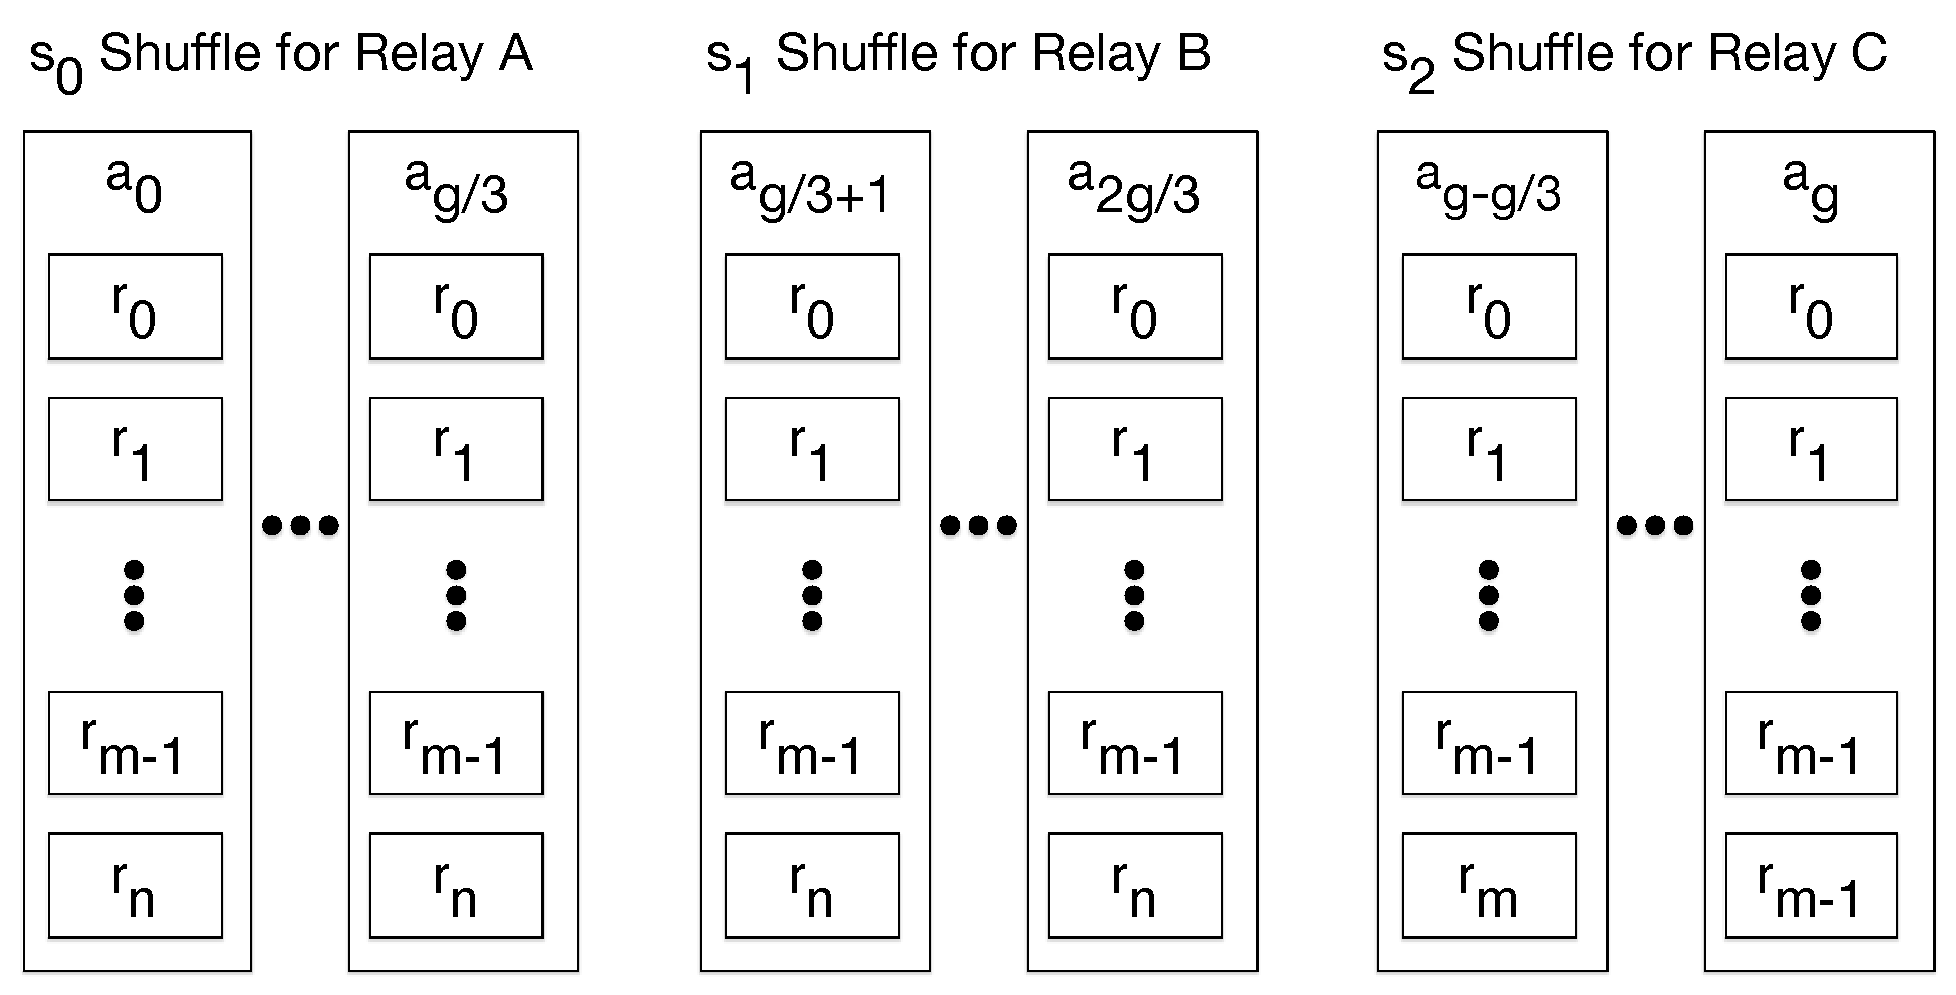
\includegraphics[scale=0.3]{torpath_shufflesets.pdf} %   \caption{Each Shuffle
% Set carries out its own Neff shuffle to determine one part of the path.} %
% \end{figure}

% % \subsubsection{TorCoin Verification} % Assignment servers input circuit
% signatures into a cryptographic accumulator, and publish that list of
% accumulators. Anyone can verify that a circuit existed at least once, simply by
% searching for a signature.

% % \subsubsection{Decoupled Protocol} % The TorPath protocol only replaces
% directory servers. Therefore, implementing it does not require modifying any Tor
% code. So clients can use the TorPath protocol for circuit assignment then
% communicate using the existing Tor protocol.

\subsection{TorCoin Mining}

In contrast with Bitcoin's reliance on proof of computation,
mining TorCoin requires proof of Tor bandwidth transfer.
In TorCoin, all participants on a circuit assigned by TorPath
may collectively mine a limited number of TorCoins, incrementally,
based on the end-to-end goodput they observe on the circuit.

\subsection{TorCoin Mining}

In contrast with Bitcoin's reliance on proof of computation,
mining TorCoin requires proof of Tor bandwidth transfer.
In TorCoin, all participants on a circuit assigned by TorPath
may collectively mine a limited number of TorCoins, incrementally,
based on the end-to-end goodput they observe on the circuit.

\subsection{TorCoin Mining}

In contrast with Bitcoin's reliance on proof of computation,
mining TorCoin requires proof of Tor bandwidth transfer.
In TorCoin, all participants on a circuit assigned by TorPath
may collectively mine a limited number of TorCoins, incrementally,
based on the end-to-end goodput they observe on the circuit.

\input{figures/tex/torcoin.tex}

\subsubsection{Proof of Bandwidth}
\begin{enumerate}
\item
Each client and relay creates a temporary key $R$
and its hash $R_*' = \textrm{Hash}(R_*)$. 

\item
Every $m$ Tor packets, the client sends a tuple $(\textrm{coin\#}, R'_C)$,
where coin\# is the number of TorCoin packets previously sent in this circuit.

\item
Each relay similarly adds its own temporary hash to the tuple --
$R'_E$, $R'_M$, and $R'_X$ --
and forwards the tuple to the next relay in the circuit.

\item
The exit relay forms the coin commitment blob
$B = (\textrm{coin\#}, R'_{C}, R'_{E}, R'_{M}, R'_{X})$.

\item
The exit relay then signs the blob $B$ with its temporary public key
for this circuit to create signature $S^B_X$,
then opens its commitment to reveal $R_X$,
and sends the tuple $(B, S^B_X, R_X)$ to the middle relay.

\item
Each prior participant in the circuit $i$, in turn,
similarly signs the blob B to create $S^B_i$,
adds its signature and opened commitment to the tuple,
then forwards the tuple to the previous participant in the circuit. 

\item
The client forms bandwidth proof
$P = (B, S^B_X, S^B_M, S^B_E, S^B_C, R_X, R_M, R_E, R_C)$,
which anyone may verify against the four temporary public keys
in the appropriate row of matrix $M$ for this circuit.

\item
To check if a TorCoin has been mined, the client checks if the lower-order
bits of $\textrm{Hash}(CS_i, B, R_X, R_M, R_E, R_C) == 0$.
If so, the client adds the full proof-of-bandwidth tuple $P$
to the blockchain to validate the new TorCoin.
To be valid,
the coin\# within $P$ must be one greater than that
of the last TorCoin in the blockchain mined from circuit $i$,
and must be less than the well-known limit on the number of TorCoins
per assigned circuit.

\item
Finally, the client uses the standard BitCoin transfer protocol
to pay each relay in the circuit one third of the mined TorCoin. 
\end{enumerate}

This protocol leaves all information necessary
for verifying proof-of-bandwidth in the blockchain.
Any interested party can verify that the circuit identifier in $B$
refers to a valid consensus group by referring to the public log.
They can also verify that the blob B was signed
by the correct participants by verifying the signatures
against the temporary public in the consensus matrix $M$,
and verify that the openings $R_i$ correspond to
the corresponding commitments $R'_i$. 
Because the low-order-bit test in step 8 depends only on values
secretly committed on the ``forward path'' in steps 2--4,
then revealed only on the ``return path'' in steps 5--6,
no proper subset of the circuit's participants can unilaterally recompute $B$
in order to mine TorCoins out of proportion to measured circuit goodput.

\subsubsection{Security Considerations}

\paragraph{Enforcing packet rate:} All honest relays and clients enforce the standard
TorCoin packet rate $m$. Any relays or clients that deviate from this are
reported to the assignment servers and the circuit is terminated.

\paragraph{Enforcing circuits:} Relays know their neighbours'
IP addresses and will refuse connections from any other IP address. Even if
malicious relays connect to each other, they will not be able to sign
TorCoins unless they own a complete circuit.

\paragraph{Compromised circuits:} Colluding clients and
attackers needs to control all four components of a circuit to mine TorCoins
fraudulently. Even if an adversary controls up to half the network,
only $1/2^4 = 1/16$ of assigned circuits will be fully colluding.
In practice, we hope and expect that 
gaining control of even half of all Tor clients and relays would be difficult.
To limit the impact of occasional colluding circuits,
TorCoin also limits the number
of coins each circuit can mine. This coin number is
included in the blockchain, so it is easily verified. 
The impact of
compromised circuits can be further reduced by ensuring that consensus groups
expire at regular intervals, requiring clients either to form new circuits
or cease obtaining new TorCoins from old circuits.

\subsubsection{Deployment:} The TorPath network is not backward compatible with
the existing Tor network, due to the fundamental differences of route
assignment and access control, which are missing in Tor but necessary for
the TorPath and TorCoin schemes to work.
However, any given physical server could run both services at the same
time. TorCoins are, of course, generated only from TorCoin traffic.


\subsubsection{Proof of Bandwidth}
\begin{enumerate}
\item
Each client and relay creates a temporary key $R$
and its hash $R_*' = \textrm{Hash}(R_*)$. 

\item
Every $m$ Tor packets, the client sends a tuple $(\textrm{coin\#}, R'_C)$,
where coin\# is the number of TorCoin packets previously sent in this circuit.

\item
Each relay similarly adds its own temporary hash to the tuple --
$R'_E$, $R'_M$, and $R'_X$ --
and forwards the tuple to the next relay in the circuit.

\item
The exit relay forms the coin commitment blob
$B = (\textrm{coin\#}, R'_{C}, R'_{E}, R'_{M}, R'_{X})$.

\item
The exit relay then signs the blob $B$ with its temporary public key
for this circuit to create signature $S^B_X$,
then opens its commitment to reveal $R_X$,
and sends the tuple $(B, S^B_X, R_X)$ to the middle relay.

\item
Each prior participant in the circuit $i$, in turn,
similarly signs the blob B to create $S^B_i$,
adds its signature and opened commitment to the tuple,
then forwards the tuple to the previous participant in the circuit. 

\item
The client forms bandwidth proof
$P = (B, S^B_X, S^B_M, S^B_E, S^B_C, R_X, R_M, R_E, R_C)$,
which anyone may verify against the four temporary public keys
in the appropriate row of matrix $M$ for this circuit.

\item
To check if a TorCoin has been mined, the client checks if the lower-order
bits of $\textrm{Hash}(CS_i, B, R_X, R_M, R_E, R_C) == 0$.
If so, the client adds the full proof-of-bandwidth tuple $P$
to the blockchain to validate the new TorCoin.
To be valid,
the coin\# within $P$ must be one greater than that
of the last TorCoin in the blockchain mined from circuit $i$,
and must be less than the well-known limit on the number of TorCoins
per assigned circuit.

\item
Finally, the client uses the standard BitCoin transfer protocol
to pay each relay in the circuit one third of the mined TorCoin. 
\end{enumerate}

This protocol leaves all information necessary
for verifying proof-of-bandwidth in the blockchain.
Any interested party can verify that the circuit identifier in $B$
refers to a valid consensus group by referring to the public log.
They can also verify that the blob B was signed
by the correct participants by verifying the signatures
against the temporary public in the consensus matrix $M$,
and verify that the openings $R_i$ correspond to
the corresponding commitments $R'_i$. 
Because the low-order-bit test in step 8 depends only on values
secretly committed on the ``forward path'' in steps 2--4,
then revealed only on the ``return path'' in steps 5--6,
no proper subset of the circuit's participants can unilaterally recompute $B$
in order to mine TorCoins out of proportion to measured circuit goodput.

\subsubsection{Security Considerations}

\paragraph{Enforcing packet rate:} All honest relays and clients enforce the standard
TorCoin packet rate $m$. Any relays or clients that deviate from this are
reported to the assignment servers and the circuit is terminated.

\paragraph{Enforcing circuits:} Relays know their neighbours'
IP addresses and will refuse connections from any other IP address. Even if
malicious relays connect to each other, they will not be able to sign
TorCoins unless they own a complete circuit.

\paragraph{Compromised circuits:} Colluding clients and
attackers needs to control all four components of a circuit to mine TorCoins
fraudulently. Even if an adversary controls up to half the network,
only $1/2^4 = 1/16$ of assigned circuits will be fully colluding.
In practice, we hope and expect that 
gaining control of even half of all Tor clients and relays would be difficult.
To limit the impact of occasional colluding circuits,
TorCoin also limits the number
of coins each circuit can mine. This coin number is
included in the blockchain, so it is easily verified. 
The impact of
compromised circuits can be further reduced by ensuring that consensus groups
expire at regular intervals, requiring clients either to form new circuits
or cease obtaining new TorCoins from old circuits.

\subsubsection{Deployment:} The TorPath network is not backward compatible with
the existing Tor network, due to the fundamental differences of route
assignment and access control, which are missing in Tor but necessary for
the TorPath and TorCoin schemes to work.
However, any given physical server could run both services at the same
time. TorCoins are, of course, generated only from TorCoin traffic.


\subsubsection{Proof of Bandwidth}
\begin{enumerate}
\item
Each client and relay creates a temporary key $R$
and its hash $R_*' = \textrm{Hash}(R_*)$. 

\item
Every $m$ Tor packets, the client sends a tuple $(\textrm{coin\#}, R'_C)$,
where coin\# is the number of TorCoin packets previously sent in this circuit.

\item
Each relay similarly adds its own temporary hash to the tuple --
$R'_E$, $R'_M$, and $R'_X$ --
and forwards the tuple to the next relay in the circuit.

\item
The exit relay forms the coin commitment blob
$B = (\textrm{coin\#}, R'_{C}, R'_{E}, R'_{M}, R'_{X})$.

\item
The exit relay then signs the blob $B$ with its temporary public key
for this circuit to create signature $S^B_X$,
then opens its commitment to reveal $R_X$,
and sends the tuple $(B, S^B_X, R_X)$ to the middle relay.

\item
Each prior participant in the circuit $i$, in turn,
similarly signs the blob B to create $S^B_i$,
adds its signature and opened commitment to the tuple,
then forwards the tuple to the previous participant in the circuit. 

\item
The client forms bandwidth proof
$P = (B, S^B_X, S^B_M, S^B_E, S^B_C, R_X, R_M, R_E, R_C)$,
which anyone may verify against the four temporary public keys
in the appropriate row of matrix $M$ for this circuit.

\item
To check if a TorCoin has been mined, the client checks if the lower-order
bits of $\textrm{Hash}(CS_i, B, R_X, R_M, R_E, R_C) == 0$.
If so, the client adds the full proof-of-bandwidth tuple $P$
to the blockchain to validate the new TorCoin.
To be valid,
the coin\# within $P$ must be one greater than that
of the last TorCoin in the blockchain mined from circuit $i$,
and must be less than the well-known limit on the number of TorCoins
per assigned circuit.

\item
Finally, the client uses the standard BitCoin transfer protocol
to pay each relay in the circuit one third of the mined TorCoin. 
\end{enumerate}

This protocol leaves all information necessary
for verifying proof-of-bandwidth in the blockchain.
Any interested party can verify that the circuit identifier in $B$
refers to a valid consensus group by referring to the public log.
They can also verify that the blob B was signed
by the correct participants by verifying the signatures
against the temporary public in the consensus matrix $M$,
and verify that the openings $R_i$ correspond to
the corresponding commitments $R'_i$. 
Because the low-order-bit test in step 8 depends only on values
secretly committed on the ``forward path'' in steps 2--4,
then revealed only on the ``return path'' in steps 5--6,
no proper subset of the circuit's participants can unilaterally recompute $B$
in order to mine TorCoins out of proportion to measured circuit goodput.

\subsubsection{Security Considerations}

\paragraph{Enforcing packet rate:} All honest relays and clients enforce the standard
TorCoin packet rate $m$. Any relays or clients that deviate from this are
reported to the assignment servers and the circuit is terminated.

\paragraph{Enforcing circuits:} Relays know their neighbours'
IP addresses and will refuse connections from any other IP address. Even if
malicious relays connect to each other, they will not be able to sign
TorCoins unless they own a complete circuit.

\paragraph{Compromised circuits:} Colluding clients and
attackers needs to control all four components of a circuit to mine TorCoins
fraudulently. Even if an adversary controls up to half the network,
only $1/2^4 = 1/16$ of assigned circuits will be fully colluding.
In practice, we hope and expect that 
gaining control of even half of all Tor clients and relays would be difficult.
To limit the impact of occasional colluding circuits,
TorCoin also limits the number
of coins each circuit can mine. This coin number is
included in the blockchain, so it is easily verified. 
The impact of
compromised circuits can be further reduced by ensuring that consensus groups
expire at regular intervals, requiring clients either to form new circuits
or cease obtaining new TorCoins from old circuits.

\subsubsection{Deployment:} The TorPath network is not backward compatible with
the existing Tor network, due to the fundamental differences of route
assignment and access control, which are missing in Tor but necessary for
the TorPath and TorCoin schemes to work.
However, any given physical server could run both services at the same
time. TorCoins are, of course, generated only from TorCoin traffic.

\section{Preliminary Results}

The TorCoin protocol adds a small amount of overhead to Tor traffic. 
To evaluate this overhead,
we set up a series of servers using the Python Twisted
framework\cite{twisted} to simulate the passing of TorCoin generation and
verification messages through a set of relays.

Assuming that the keys, hashes and signatures are all 32 bytes in length,
the total overhead from one round of successful TorCoin mining (i.e., one entire
round trip from client through all the relays and back again) results in a total
TorCoin packet overhead of 814 bytes. This can be broken down into:

\begin{itemize}
	\item The first packet from client to entry relay: 34 bytes.
	\item Packet forwarded from entry to middle relay: 66 bytes.
	\item Packet forwarded from middle to exit relay: 98 bytes.
	\item Packet from from exit to middle relay: 164 bytes.
	\item Packet from from middle to entry relay: 194 bytes.
	\item Packet from from entry relay to client: 258 bytes.
	\item Total: 814 bytes
\end{itemize}

\section{Preliminary Results}

The TorCoin protocol adds a small amount of overhead to Tor traffic. 
To evaluate this overhead,
we set up a series of servers using the Python Twisted
framework\cite{twisted} to simulate the passing of TorCoin generation and
verification messages through a set of relays.

Assuming that the keys, hashes and signatures are all 32 bytes in length,
the total overhead from one round of successful TorCoin mining (i.e., one entire
round trip from client through all the relays and back again) results in a total
TorCoin packet overhead of 814 bytes. This can be broken down into:

\begin{itemize}
	\item The first packet from client to entry relay: 34 bytes.
	\item Packet forwarded from entry to middle relay: 66 bytes.
	\item Packet forwarded from middle to exit relay: 98 bytes.
	\item Packet from from exit to middle relay: 164 bytes.
	\item Packet from from middle to entry relay: 194 bytes.
	\item Packet from from entry relay to client: 258 bytes.
	\item Total: 814 bytes
\end{itemize}

\section{Preliminary Results}

The TorCoin protocol adds a small amount of overhead to Tor traffic. 
To evaluate this overhead,
we set up a series of servers using the Python Twisted
framework\cite{twisted} to simulate the passing of TorCoin generation and
verification messages through a set of relays.

Assuming that the keys, hashes and signatures are all 32 bytes in length,
the total overhead from one round of successful TorCoin mining (i.e., one entire
round trip from client through all the relays and back again) results in a total
TorCoin packet overhead of 814 bytes. This can be broken down into:

\begin{itemize}
	\item The first packet from client to entry relay: 34 bytes.
	\item Packet forwarded from entry to middle relay: 66 bytes.
	\item Packet forwarded from middle to exit relay: 98 bytes.
	\item Packet from from exit to middle relay: 164 bytes.
	\item Packet from from middle to entry relay: 194 bytes.
	\item Packet from from entry relay to client: 258 bytes.
	\item Total: 814 bytes
\end{itemize}

\input{figures/tex/results.tex}

Each round of TorCoin generation and verification happens only after $m$ Tor
packets have been sent. Each standard Tor cell is 514 bytes long, so each
round trip on the network requires transmission of 514 * 6 = 3084 bytes. Thus,
if $m \geq 10$, the TorCoin protocol overhead is around 2\%. The value of $m$
can be calibrated in further experimentation and as needed in order to achieve
the sweet-spot of transmission efficiency and incentive maximization for relay
providers.

The system might decrease the value of $m$ when load is high,
incentivizing relay operators
to provision more relay bandwidth at such times.

While the Neff shuffle is complex and requires several
communications between the servers,
we expect the assignment servers will be few (less than 10)
and well-provisioned,
and do not expect the shuffles to be a major bottleneck.
Since this is a one-time cost of connecting to the network,
we hope users will accept this setup time
if it gives them access to higher-capacity relays.
For impatient users,
the TorCoin client could use conventional Tor circuits immediately on startup,
then transition to TorCoin circuits as they become available.



Each round of TorCoin generation and verification happens only after $m$ Tor
packets have been sent. Each standard Tor cell is 514 bytes long, so each
round trip on the network requires transmission of 514 * 6 = 3084 bytes. Thus,
if $m \geq 10$, the TorCoin protocol overhead is around 2\%. The value of $m$
can be calibrated in further experimentation and as needed in order to achieve
the sweet-spot of transmission efficiency and incentive maximization for relay
providers.

The system might decrease the value of $m$ when load is high,
incentivizing relay operators
to provision more relay bandwidth at such times.

While the Neff shuffle is complex and requires several
communications between the servers,
we expect the assignment servers will be few (less than 10)
and well-provisioned,
and do not expect the shuffles to be a major bottleneck.
Since this is a one-time cost of connecting to the network,
we hope users will accept this setup time
if it gives them access to higher-capacity relays.
For impatient users,
the TorCoin client could use conventional Tor circuits immediately on startup,
then transition to TorCoin circuits as they become available.



Each round of TorCoin generation and verification happens only after $m$ Tor
packets have been sent. Each standard Tor cell is 514 bytes long, so each
round trip on the network requires transmission of 514 * 6 = 3084 bytes. Thus,
if $m \geq 10$, the TorCoin protocol overhead is around 2\%. The value of $m$
can be calibrated in further experimentation and as needed in order to achieve
the sweet-spot of transmission efficiency and incentive maximization for relay
providers.

The system might decrease the value of $m$ when load is high,
incentivizing relay operators
to provision more relay bandwidth at such times.

While the Neff shuffle is complex and requires several
communications between the servers,
we expect the assignment servers will be few (less than 10)
and well-provisioned,
and do not expect the shuffles to be a major bottleneck.
Since this is a one-time cost of connecting to the network,
we hope users will accept this setup time
if it gives them access to higher-capacity relays.
For impatient users,
the TorCoin client could use conventional Tor circuits immediately on startup,
then transition to TorCoin circuits as they become available.


%\section{Discussion} \label{disc}

\todo[this section is currently merely an outline of topics for discussion]

\subsection{Path to Deployment}

If it is run outside of Tor it may be better for experimental purposes, but longer term it would be nice not to partition the network.

How do these options this affect the anonymity sets? Will it always be possible to split the sets anyway due to the fundamental nature of diffserv scheduling?

\subsubsection{Deploy in Existing Tor Network}

Write Tor proposals, get all the new features blessed by the Tor developers, integrate into existing network.

\subsubsection{New and Separate Anonymity Network}

Fork Tor and add the new features. Create a separate network that does not interact with the existing network.

\subsubsection{New Anonymity Network used with Tor}

Run a separate network that is 'attached' to the existing network. In other words, the new network interoperates with Tor by having two consensus files, etc. Then, when people wanting to use the coin mechanism use the new consensus to choose relays from the new network, and non-payers use the Tor consensus to choose circuits in the existing Tor network.

As it is important to minimize the loss in anonymity to the existing Tor users,
we propose the deployment of a secondary experimental Tor network that will
separate the incentive design and its risks from the existing network. Those
participating in the incentive scheme will choose relays from a new consensus
produced by a new set of directory servers, and those that do not with to
participate will use the existing network as usual. This deployment strategy
offers the flexibility of merging the incentive design back into Tor should it
prove beneficial, while minimizing risk should it not.

\subsection{Trust in Network Elements}

The benefits of a system that is capable of moving to a decentralized trust model.

\subsubsection{Federated}

\begin{itemize}
\item runs on existing directory servers using something like opentransactions.org to provide ecash
\item transactions are instantaneous
\item relies on small trusted directory server set
\item communication/performance overhead among bank members means it is not scalable, and it gets more complicated if you need several federated sets to handle different parts of the network
\end{itemize}

\subsubsection{Completely decentralized}

\begin{itemize}
\item use an AltCoin or something else as a distributed storage medium for the ledger
\item more scalable
\item decentralized trust may not be relevant in Tor's existing trust model, but will be when Tor moves away from federated directory server model
\item transaction linkability issues leads to protocol complexities and questions about anonymity. does zerocoin work here?
\end{itemize}

\subsection{Diversity}

\subsubsection{Location Diversity}

The market might prefer a single cheap ISP, which would not add additional location diversity to the network. Could we create a "diversity weight" and pay more for relays that increase the diversity weight?

\subsubsection{Circuit Position Diversity}

Should we pay more for entry or exit position, or for exit policies that are more open by some definition? Or will the market smooth this out automatically?

\subsubsection{Diversity in Capabilities}

Could we offer more reward for faster relays (i.e. a super-linear reward scale)?  Or for relays that are running a certain version or support a certain feature (experimental or otherwise)? This could improve the community's ability to contribute to decisions about what to support instead of completely relying on the Tor developers (could be a good thing or a bad thing).

\subsection{Community}

If a new incentive scheme is incorporated into Tor, will existing volunteers stop caring become less altruistic and leave because they will view Tor as a commercial network? Will people lose interest in helping the broader Internet freedom cause?

Does a token that only provides a performance enhancement but has no intrisic value (cannot be traded with others) solve this problem? Or does the fact that you can trade the coins provide most of the incentives?

Would a smaller scale experiment outside of the existing Tor network to test the feasibility of an incentive approach be helpful, or would the conclusions simply be synthetic because users/relays in the experimental network would not have the same ideals and values as in existing network?
\section{Related Work} \label{rel}

PAR~\cite{raykova-pet2008}, XPay~\cite{wpes09-xpay}, Gold Star~, BRAIDS~\cite{ccs10-braids}, Tortoise~, onions for sale~\cite{johnson2013onions}.

On the economics of anonymity~\cite{Acquisti03onthe}, one-to-n scrip systems~\cite{humbert2011-scrip}.

LIRA~\cite{jansen2013lira}is a lightweight system providing “performance incentives for users to contribute bandwidth to the Tor network.” It uses coins, similar to “in game currency,” to distribute payment. LIRA uses coins which have a tunable probability of being right, and clients can guess lottery tickets with probability, p of being right. 

Eigenspeed~\cite{snader2009eigenspeed} is a peer-to-peer consensus building algorithm for monitoring bandwidth over a network, specifically implemented for Tor. Unfortunately it requires a central authority for computing Principal Component Analysis operations. While we believe these operations could be decentralized, we are not interested in extending Eigenspeed. Instead, we exploit properties of the Bitcoin protocol to allow for bandwidth monitoring that is sufficient to generate payment tickets. However, as mentioned before, Eigenspeed could act as a secondary system to monitor relays and clients that seem to be producing more TorCoins than would be warranted by their speed.  
\section{Conclusions} \label{conc}

We have introduced TorPath, a novel scheme to assign paths to Tor
clients securely and anonymously.
TorPath motivated by the need to verifiably mine TorCoins, a
a BitCoin variant based on measured bandwidth over the Tor network.
The TorCoin protocol is robust to malicious relays and clients
colluding to mint TorCoins without transferring bandwidth.

\com{	This is a very minor optimization,
	not worth mentioning if it's the only "Future Work" listed. -baf
Further work could investigate the use of cryptographic accumulators for circuit
signatures, which could reduce the packet overhead during bandwidth-measurement
and make the protocol more efficient.
}

\subsection*{Acknowledgments}

This material is based upon work supported by the Defense Advanced Research
Agency (DARPA) and SPAWAR Systems Center Pacific, Contract No. N66001-11-C-4018.
This work was supported by the Office of Naval Research.



{ \footnotesize %\scriptsize %\footnotesize %\small
\bibliographystyle{styles/splncs}
\balance\bibliography{references}
}

%\clearpage
% \appendix
%\appendixpage
\section*{Appendices}

\section{Performance Rewards with Differentiated Services}

We now describe how the differentiated services
architecture~\cite{blake1998architecture} can be used to improve the control
over traffic priority in Tor, as previously outlined by
Jansen~\cite{jansenphdthesis}. More specifically, the proportional
differentiation model~\cite{dovrolis1999case} allows for predictable (i.e.,
consistent as load increases) and controllable (i.e., adjustable differentiation) performance between N traffic
classes. The model allows for the configuration of a differentiation parameter
$p_i$ for each class $i$, and enforces the proportional priority of a traffic
quality metric $q$ between all pairs of classes $i$ and $j$ for measurement
timescale $\sigma$ as:
\begin{equation}
\forall i \in [N], \forall j \in [N]: \frac{q_i \left( t, t + \sigma \right)}{q_j \left( t, t + \sigma \right)} = \frac{p_i}{p_j}
\end{equation}
where $p_1 < ... < p_N$ and $p_i/p_j$ defines the quality proportion between
classes $i$ and $j$. The model is well defined when there is enough
traffic in each class to allow a work-conserving scheduler to meet the desired
proportions.

Dovrolis \etal design a scheduler under the proportional differentiation model
using a queuing delay metric~\cite{dovrolis2002proportional}, which in our case
corresponds to Tor cell waiting times. For class $i$, the quality metric $q_i$
combines the queuing delay $D_i(t)$ of the longest waiting cell with the
long-term average delay $\delta_i(t)$  of all previously scheduled cells at time $t$:
\begin{equation}
q_i(t) = D_i(t) \cdot f + \delta_i(t) \cdot (1-f)
\end{equation}
where $f$ is an adjustable fraction that tunes the schedulers ability to react
to short term spikes in delay. When a scheduling decision is to be made at time $t$,
the longest waiting cell from the class with the maximum priority
$P(t) = q(t)/p(t)$ is chosen and scheduled.


Todo - DRAFT NOTES:

This section will detail the economic model and present any lingering questions. There will be another diagram featuring multiple clients, a PSP, and multiple hosts. The diagram below will go into the software architecture section, under a section called ``system design'', followed by a sentence describing each component. Then we will go into detail on the ephemeral paths and TorCoin design, which are part of the TorCoin Minter. The TorCoin trader, wallet, and exchange are all necessary, but not novel in terms of design, so we will spend little time on those.

TODO: Add component to Client, ``TorCoin Minter'' (?)

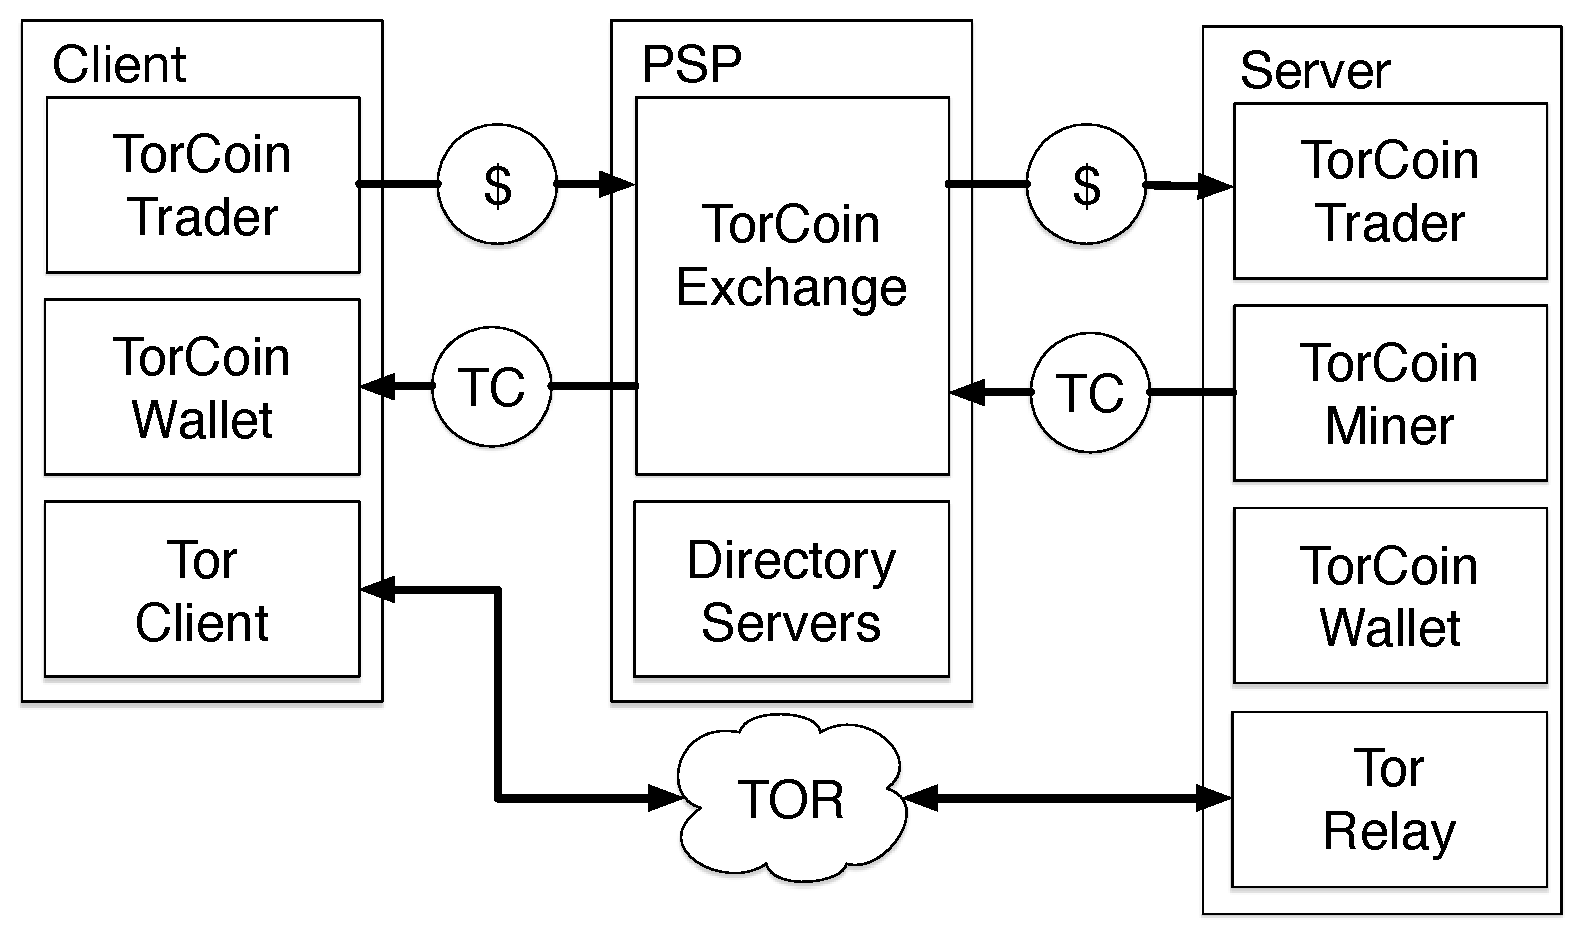
\includegraphics[scale=0.5]{figures/overview.pdf}

\end{document}
